\begin{frame}{Contents}
\tableofcontents
\end{frame}

\begin{frame}{Introduction}
    \begin{itemize}
      \item We use spatial filtering to enhance images, e.g., noise filtering. We can use the same technique to locate objects in images, called template matching. After completing this lesson, we would be able to process images using filters, as done in popular image processing software such as Photoshop.
      \item Intensity transformations affect the brightness (intensity level)of an image. The resulting value of a pixel after an intensity operation is just dependent on the original value of the same pixel.
      \item In contrast, the resulting value of a pixel after a spatial filtering operation depends on the neighborhood of the pixel in question. So the space around the pixel in question matters, hence, the name spatial filtering.
      \item In linear spatial filtering we use the 2-D convolution operation.
    \end{itemize}
\end{frame}

\begin{frame}
        \begin{figure}
          \centering
            \begin{tikzpicture}[x=0.7cm, y=0.7cm]
%Ranga Rodrigo
%September 11, 2019


\def\rows{6}
\def\cols{7}
\def\linecol{blue!60}

% Kernel only
\draw[thick, \linecol] (0,7) rectangle ++(3,3);
\draw[thick, \linecol] (0,8) rectangle ++(3,1);
\draw[thick, \linecol] (1,7) rectangle ++(1,3);

\foreach \i in {0,1,2}
{
	\foreach \j in {0,1,2}
	{
		\node at (\i + 0.5, \j + 7.5) {\scriptsize $\frac{1}{9}$};
	}
}

\begin{filecontents*}{./Figures/interpimage.dat}
0
0
0
0
0
0
0

0
0
0
0
0
0
0

0
0
180
90
180
180
0

0
0
180
90
90
180
90

0
0
0
0
0
0
0

0
0
0
0
0
0
0
\end{filecontents*}


\begin{filecontents*}{./Figures/convout.dat}
20
30
40
40
40

40
60
90
90
80

40
60
90
90
80

20
30
50
50
40

x
x
x
x
x
\end{filecontents*}



% Image grid
\def\printindices{true}
\def\printimagevalues{true}
\foreach \i in {0,1, ..., \rows}
{
	\draw[black] (0, \i)  -- ++(\cols, 0);
}
\foreach \j in {0,1, ..., \cols}
{
	\draw[black] (\j, 0)  -- ++(0, \rows);
}


\pgfmathsetmacro{\rowsminusone}{\rows -1 }%
\pgfmathsetmacro{\colsminusone}{\cols -1 }%
\pgfmathsetmacro{\rowsminustwo}{\rows -2 }%
\pgfmathsetmacro{\colsminustwo}{\cols -2 }%

\ifthenelse{\equal{\printindices}{true}}
{
	\foreach \i in {0,1, ..., \rowsminusone}
	{
			\node at (-0.5, \rowsminusone - \i + 0.5) {\scriptsize{\i}};
	}
	
	\foreach \j in {0,1, ..., \colsminusone}
	{
			\node at (\j + 0.5, \rows + 0.5) {\scriptsize{\j}};
	}
}
{}

\ifthenelse{\equal{\printimagevalues}{true}}
{
	\pgfplotstableread{./Figures/interpimage.dat}{\imagevalues}
	
	\foreach \i in {0,1, ..., \rowsminusone}
	{
		\foreach \j in {0,1, ..., \colsminusone}
		{	
			\pgfmathsetmacro{\index}{\i*\cols+\j}%
			\pgfplotstablegetelem{\index}{[index] 0}\of{\imagevalues}%
			\let\imagevalue\pgfplotsretval%
			 \node at (\j + 0.5,  \i + 0.5) {\scriptsize {\imagevalue}};
		}
	}
}
{}


% Result grid
\def\printindices{true}
\def\printimagevalues{true}
\foreach \i in {0,1, ..., \rows}
{
	\draw[black] (8, \i )  -- ++(\cols, 0);
}
\foreach \j in {0,1, ..., \cols}
{
	\draw[black] (\j + 8, 0)  -- ++(0, \rows);
}


\pgfmathsetmacro{\rowsminusone}{\rows -1 }%
\pgfmathsetmacro{\colsminusone}{\cols -1 }%


\ifthenelse{\equal{\printindices}{true}}
{
	\foreach \i in {0,1, ..., \rowsminusone}
	{
			\node at (7.5, \rowsminusone - \i + 0.5) {\scriptsize{\i}};
	}
	
	\foreach \j in {0,1, ..., \colsminusone}
	{
			\node at (\j + 8.5, \rows + 0.5) {\scriptsize{\j}};
	}
}
{}


\pgfplotstableread{./Figures/convout.dat}{\convouts}

% Kernel grid
\foreach \i in {0, 1, 2, 3}%
{
	\foreach \j in {0,1, ..., 4}% 	
	{
			\draw[\linecol, thick] (\j,  3 - \i) rectangle ++ (3,3);
			\draw[\linecol, thick] (\j, 4-\i) rectangle ++(3,1);
			\draw[\linecol, thick] (\j+1, 3-\i) rectangle ++(1,3);
            \draw[red, thick] (\j+1, 4-\i) rectangle ++(1,1);
			\draw[draw=none, fill=green!20, opacity=0.2] (\j+1, 4- \i) rectangle ++(1,1);
			\pgfmathsetmacro{\index}{\i*5+\j}%
			\pgfplotstablegetelem{\index}{[index] 0}\of{\convouts}%
			\let\convout\pgfplotsretval%
			 \node at (\j + 9.5,  4.5- \i) {\scriptsize {\convout}};
            \pause;
	}
}


\end{tikzpicture}

          \caption{Convolution}
        \end{figure}
\end{frame}



\begin{frame}{Examples of Effect of Kernel Choices}
    \begin{columns}[t]
        \column{0.7\textwidth}
        \begin{figure}
            \centering
            \begin{subfigure}[b]{0.45\textwidth}
                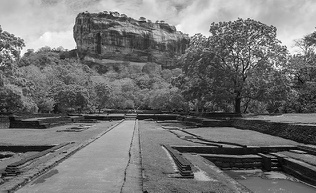
\includegraphics[width=\textwidth]{./figures/sigiriya.jpg}
                \caption{Original}
                \label{sfi:sigiriya_original}
            \end{subfigure}
            \hspace{0.2cm}
            \begin{subfigure}[b]{0.45\textwidth}
                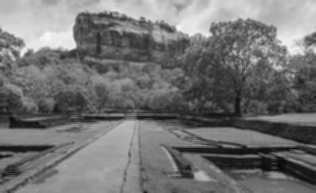
\includegraphics[width=\textwidth]{./figures/sigiriya_averaged.jpg}
                \caption{Avegaging}
                \label{sfi:sigiriya_averaged}
            \end{subfigure}\\
            \centering
            \begin{subfigure}[b]{0.45\textwidth}
                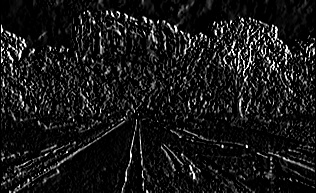
\includegraphics[width=\textwidth]{./figures/sigiriya_sobel_horizontal.jpg}
                \caption{Sobel horizontal}
                \label{sfi:sigiriya_sobel_horizontal}
            \end{subfigure}
            \hspace{0.2cm}
            \begin{subfigure}[b]{0.45\textwidth}
                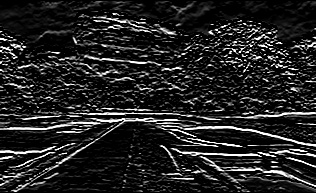
\includegraphics[width=\textwidth]{./figures/sigiriya_sobel_vertical.jpg}
                \caption{Sobel vertical}
                \label{sfi:sigiriya_averaged}
            \end{subfigure}
            \caption{Effect of kernels.}\label{fi:effect_of_kernels}
        \end{figure}
        \column{0.3\textwidth}
        \begin{figure}
            \centering
            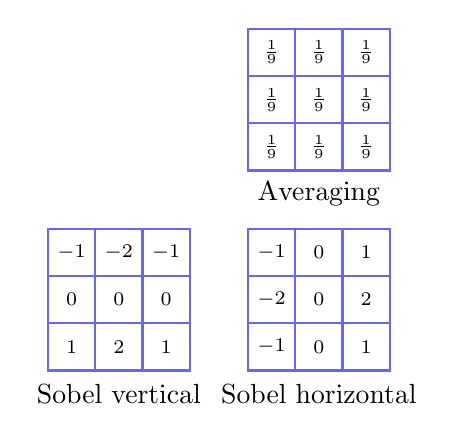
\begin{tikzpicture}[x=0.6cm, y=0.6cm]
%Ranga Rodrigo
%September 11, 2019


\def\rows{6}
\def\cols{7}
\def\linecol{blue!60}

\begin{filecontents*}{./sobelv.dat}
-1
-2
-1
0
0
0
1
2
1
\end{filecontents*}


\begin{filecontents*}{./sobelh.dat}
-1
0
1
-2
0
2
-1
0
1
\end{filecontents*}


\begin{scope}[xshift=1in]
% Kernel only
\draw[thick, \linecol] (0,0) rectangle ++(3,3);
\draw[thick, \linecol] (0,1) rectangle ++(3,1);
\draw[thick, \linecol] (1,0) rectangle ++(1,3);

\foreach \i in {0,1,2}
{
	\foreach \j in {0,1,2}
	{
		\node at (\i + 0.5, \j + 0.5) {\scriptsize $\frac{1}{9}$};
	}
}
\node at (1.5, -0.5) {Averaging};
\end{scope}

\begin{scope}[yshift=-1in]
% Kernel only
\draw[thick, \linecol] (0,0) rectangle ++(3,3);
\draw[thick, \linecol] (0,1) rectangle ++(3,1);
\draw[thick, \linecol] (1,0) rectangle ++(1,3);

\pgfplotstableread{./sobelv.dat}{\sobelvs}
	
	\foreach \i in {0,1, 2}
	{
		\foreach \j in {0,1, 2}
		{	
			\pgfmathsetmacro{\index}{\i*3+\j}%
			\pgfplotstablegetelem{\index}{[index] 0}\of{\sobelvs}%
			\let\sobelv\pgfplotsretval%
			\node at (\j + 0.5, 2.5 - \i) {\scriptsize $\sobelv$};
	}
}
\node at (1.5, -0.5) {Sobel vertical};
\end{scope}

\begin{scope}[xshift=1in, yshift=-1in]
% Kernel only
\draw[thick, \linecol] (0,0) rectangle ++(3,3);
\draw[thick, \linecol] (0,1) rectangle ++(3,1);
\draw[thick, \linecol] (1,0) rectangle ++(1,3);

\pgfplotstableread{./sobelh.dat}{\sobelhs}
	
	\foreach \i in {0,1, 2}
	{
		\foreach \j in {0,1, 2}
		{	
			\pgfmathsetmacro{\index}{\i*3+\j}%
			\pgfplotstablegetelem{\index}{[index] 0}\of{\sobelhs}%
			\let\sobelh\pgfplotsretval%
			\node at (\j + 0.5, 2.5 - \i) {\scriptsize $\sobelh$};
	}
}
\node at (1.5, -0.5) {Sobel horizontal};
\end{scope}


\end{tikzpicture}

            \caption{$3\times 3$ kernels}
            \label{fi:kernels}
        \end{figure}
    \end{columns}

\end{frame}

\begin{frame}[t, fragile]{Spatial Filtering (Averaging) Using \lstinline!filter2D!}
    \begin{lstlisting}[caption=Spatial Filtering (Averaging), language=Python, escapechar=\@]
%matplotlib inline
import cv2 as cv
import numpy as np
from matplotlib import pyplot as plt

img = cv.imread('../images/sigiriya.jpg', cv.IMREAD_REDUCED_GRAYSCALE_2)

kernel = np.ones((3,3),np.float32)/9
imgc = cv.filter2D(img,-1,kernel)

fig, axes  = plt.subplots(1,2, sharex='all', sharey='all', figsize=(18,18))
axes[0].imshow(img, cmap='gray')
axes[0].set_title('Original')
axes[0].set_xticks([]), axes[0].set_yticks([])
axes[1].imshow(imgc, cmap='gray')
axes[1].set_title('Averaging')
axes[1].set_xticks([]), axes[1].set_yticks([])
plt.show()
    \end{lstlisting}
\end{frame}

\begin{frame}[t, fragile]{Spatial Filtering (Sobel Vertical) Using \lstinline!filter2D!}
    \begin{lstlisting}[caption=Spatial Filtering (Sobel Vertical), language=Python, escapechar=\@]
%matplotlib inline
import cv2 as cv
import numpy as np
from matplotlib import pyplot as plt

img = cv.imread('../images/sigiriya.jpg', cv.IMREAD_REDUCED_GRAYSCALE_2)

kernel = np.array([(-1, -2, -1), (0, 0, 0), (1, 2, 1)], dtype='float')
imgc = cv.filter2D(img,-1,kernel)

fig, axes  = plt.subplots(1,2, sharex='all', sharey='all', figsize=(18,18))
axes[0].imshow(img, cmap='gray')
axes[0].set_title('Original')
axes[0].set_xticks([]), axes[0].set_yticks([])
axes[1].imshow(imgc, cmap='gray')
axes[1].set_title('Averaging')
axes[1].set_xticks([]), axes[1].set_yticks([])
plt.show()
    \end{lstlisting}
\end{frame}


\begin{frame}{Convolution and Correlation}
    \begin{enumerate}
        \item Spatial filtering is, in fact, convolution.
        \item As the filters are typically symmetric---i.e., a $180^\circ$ rotation results in the same kernel---correlation is equivalent to convolution.
        \item Correlation is also the scalar product between the kernel and the underlying image patch. Therefore, it is a measure of similarity between the kernel and the underlying image patch.
        \item As a result, when the kernel and the patch are ``similar'', the output is high. In view of this, spatial filtering seeks for patches in the image that are similar  to the kernel.
        \item Implementing filtering using loops (four nested for loops) in a non-C fashion is inefficient. Instead, use \lstinline!filter2D!.
    \end{enumerate}
\end{frame}


\begin{frame}{Convolution and Correlation}
    The convolution sum expression that we leaned in signal and systems is
    \begin{equation*}\label{eq:1d_conv_sum}
        y[n] = x[n]\ast h[n] = \sum_{k=-\infty}^{\infty}x[k]h[n-k].
    \end{equation*}
    In 2-D, as applicable in image processing, collation sum with a kernel $w[m,n]$ with non-zero values in $(m,n) \in ([-a,a], [-b,b])$ is
    \begin{equation*}\label{eq:2d_conv_sum}
        (w\ast f)[m,n] = w[m,n]\ast f[m,n] = \sum_{s=-a}^{a}\sum_{k=-b}^{b} w[s,t]f[m-s, n-t].
    \end{equation*}
    Correlation:
    \begin{equation*}\label{eq:2d_conv_sum}
        (w\circledast f)[m,n] = w[m,n]\circledast f[m,n] = \sum_{s=-a}^{a}\sum_{k=-b}^{b} w[s,t]f[m+s, n+t].
    \end{equation*}
\end{frame}

\begin{frame}[t, fragile, allowframebreaks]{}
    \begin{lstlisting}[caption=Filtering Using Loops, language=Python, escapechar=\@]
%matplotlib inline
import cv2 as cv
import matplotlib.pyplot as plt
import numpy as np
import math

def filter(image, kernel):
    assert kernel.shape[0]%2 == 1 and kernel.shape[1]%2 == 1
    k_hh, k_hw = math.floor(kernel.shape[0]/2), math.floor(kernel.shape[1]/2)
    h, w = image.shape
    image_float = cv.normalize(image.astype('float'), None, 0.0, 1.0, cv.NORM_MINMAX)
    result = np.zeros(image.shape, 'float')

    for m in range(k_hh, h - k_hh):
        for n in range(k_hw, w - k_hw):
            result[i,j] = np.dot(image_float[m-k_hh:m + k_hh + 1, n - k_hw : n + k_hw + 1].flatten(), kernel.flatten())
    return result

img = cv.imread('../images/keira.jpg', cv.IMREAD_REDUCED_GRAYSCALE_8)
f, axarr = plt.subplots(1,2)
axarr[0].imshow(img, cmap="gray")
axarr[0].set_title('Original')
kernel = np.array([(1/9, 1/9, 1/9), (1/9, 1/9, 1/9), (1/9, 1/9, 1/9)], dtype='float')
imgb = filter(img, kernel)
imgb = imgb*255.0
imgb = imgb.astype(np.uint8)

axarr[1].imshow(imgb, cmap="gray")
axarr[1].set_title('Filtered')
    \end{lstlisting}
\end{frame}

\begin{frame}{Example}
    Consider the image
    \begin{equation*}
        f = \begin{bmatrix}
          0 & 0 & 0 & 0 & 0\\
          0 & 0 & 0 & 0 & 0\\
          0 & 0 & 1 & 0 & 0\\
          0 & 0 & 0 & 0 & 0\\
          0 & 0 & 0 & 0 & 0\\
        \end{bmatrix}
    \end{equation*}
    and the filtering kernel
    \begin{equation*}
        w = \begin{bmatrix}
          1 & 2 & 3\\
          4 & 5 & 6\\
          7 & 8 & 9\\
        \end{bmatrix}
    \end{equation*}.
    Appropriately pad the image. Carry out a. correlation b. convolution.
\end{frame}


\begin{frame}{Solution}%<beamer>
    Consider the image
    \begin{equation*}
        f_\mathrm{padded} = \begin{bmatrix}
          0 & 0 & 0 & 0 & 0 & 0 & 0\\
          0 & 0 & 0 & 0 & 0 & 0 & 0\\
          0 & 0 & 0 & 0 & 0 & 0 & 0\\
          0 & 0 & 0 & 1 & 0 & 0 & 0\\
          0 & 0 & 0 & 0 & 0 & 0 & 0\\
          0 & 0 & 0 & 0 & 0 & 0 & 0\\
          0 & 0 & 0 & 0 & 0 & 0 & 0\\
        \end{bmatrix}
        \qquad
        w = \begin{bmatrix}
          1 & 2 & 3\\
          4 & 5 & 6\\
          7 & 8 & 9\\
        \end{bmatrix}
    \end{equation*}
    Correlation result and convolution result, respectively
    \begin{equation*}
        (w\circledast f) = \begin{bmatrix}
          0 & 0 & 0 & 0 & 0\\
          0 & 9 & 8 & 7 & 0\\
          0 & 6 & 5 & 4 & 0\\
          0 & 3 & 2 & 1 & 0\\
          0 & 0 & 0 & 0 & 0\\
        \end{bmatrix}\qquad
        (w\ast f) = \begin{bmatrix}
          0 & 0 & 0 & 0 & 0\\
          0 & 1 & 2 & 3 & 0\\
          0 & 4 & 5 & 6 & 0\\
          0 & 7 & 8 & 9 & 0\\
          0 & 0 & 0 & 0 & 0\\
        \end{bmatrix}
    \end{equation*}.
\end{frame}

\begin{frame}{Convolution: Key Properties}
    \begin{enumerate}
        \item Linearity: $\mathrm{filter}(f_1 + f_2) = \mathrm{filter}(f_1) + \mathrm{filter}(f_2)$
        \item Shift invariance: same behavior regardless of pixel location: $\mathrm{filter}(\mathrm{shift}(f)) = \mathrm{shift}(\mathrm{filter}(f))$
        \item Theoretical result: any linear shift-invariant operator can be represented as a convolution.
    \end{enumerate}
    Other Properties
    \begin{enumerate}
        \item Commutative: $a \ast b = b \ast a$
        \item Conceptually no difference between filter and signal
        \item Associative: $a \ast (b \ast c) = (a \ast b) \ast c$
        \item Often apply several filters one after another: $(((a \ast b_1) \ast b_2) \ast b_3)$
        \item This is equivalent to applying one filter: $a \ast (b_1 \ast b_2 \ast b_3)$
        \item Distributes over addition: $a \ast (b + c) = (a \ast b) + (a \ast c)$
        \item Scalars factor out: $ka \ast b = a \ast kb = k (a \ast b)$
        \item Identity: unit impulse $e = [\dots, 0, 0, 1, 0, 0, \dots]$, $a \ast e = a$
    \end{enumerate}

    \credit{Svetlana Lazebnik}
\end{frame}


\begin{frame}{At the Edge}
    \begin{enumerate}
        \item The filter window falls off the edge of the image.
        \item Need to extrapolate the image.
        \item Methods: various border types, image boundaries are denoted with '|'
        \begin{tabular}{lcl}
            \lstinline!BORDER_REPLICATE:! & \texttt{aaaaaa|abcdefgh|hhhhhhh}&\\
            \lstinline!BORDER_REFLECT:! & \texttt{fedcba|abcdefgh|hgfedcb}&\\
            \lstinline!BORDER_REFLECT_101:! & \texttt{gfedcb|abcdefgh|gfedcba}&\\
            \lstinline!BORDER_WRAP:! &         \texttt{cdefgh|abcdefgh|abcdefg}&\\
            \lstinline!BORDER_CONSTANT:! &      \texttt{iiiiii|abcdefgh|iiiiiii}&  with some specified 'i'\\
        \end{tabular}
    \end{enumerate}
\end{frame}




% Four Pictures
\begin{frame}{Sharpening}
    \begin{figure}
        \centering
        \begin{subfigure}[b]{0.25\textwidth}
            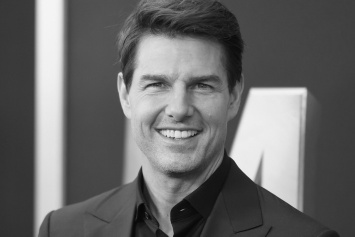
\includegraphics[width=\textwidth]{./figures/sharpening_original.jpg}
            \caption{Original}
            \label{sfi:sharpening_original}
        \end{subfigure}
        \begin{subfigure}[b]{0.05\textwidth}
            \centering
            $-$
            \vspace{2cm}
        \end{subfigure}
        \begin{subfigure}[b]{0.25\textwidth}
            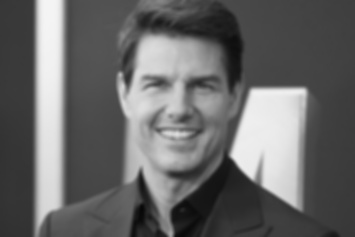
\includegraphics[width=\textwidth]{./figures/sharpening_blurred.jpg}
            \caption{Smoothed}
            \label{sfi:sharpening_blurred}
        \end{subfigure}
        \begin{subfigure}[b]{0.05\textwidth}
            \centering
            $=$
            \vspace{2cm}
        \end{subfigure}
        \begin{subfigure}[b]{0.25\textwidth}
            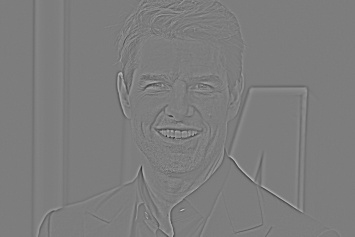
\includegraphics[width=\textwidth]{./figures/sharpening_diff.jpg}
            \caption{Original $-$ Smoothed}
            \label{sfi:sharpening_diff}
        \end{subfigure}\\
        \centering
        \begin{subfigure}[b]{0.25\textwidth}
            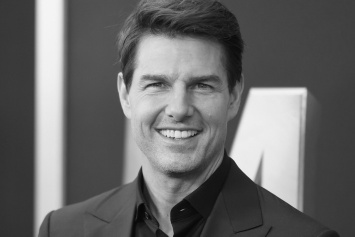
\includegraphics[width=\textwidth]{./figures/sharpening_original.jpg}
            \caption{Original}
            \label{sfi:sharpening_original_1}
        \end{subfigure}
        \begin{subfigure}[b]{0.05\textwidth}
            \centering
            $-$
            \vspace{2cm}
        \end{subfigure}
        \begin{subfigure}[b]{0.25\textwidth}
            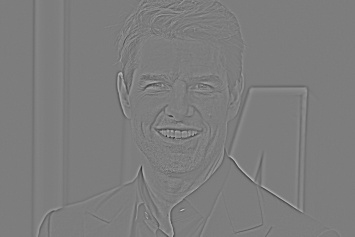
\includegraphics[width=\textwidth]{./figures/sharpening_diff.jpg}
            \caption{Original $-$ Smoothed}
            \label{sfi:sharpening_diff_1}
        \end{subfigure}
        \begin{subfigure}[b]{0.05\textwidth}
            \centering
            $=$
            \vspace{2cm}
        \end{subfigure}
        \begin{subfigure}[b]{0.25\textwidth}
            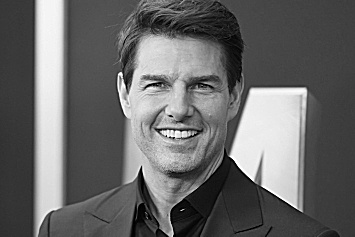
\includegraphics[width=\textwidth]{./figures/sharpening_sharpened.jpg}
            \caption{Sharpened}
            \label{sfi:sharpening_sharpened}
        \end{subfigure}\\
        \caption{Sharpening (125 added to Original $-$ Smoothed to display)}\label{fi:effect_of_kernels}
    \end{figure}
    \credit{Svetlana Lazebnik}
\end{frame}


\begin{frame}{Box Filter vs. Gaussian Filter}
    \begin{itemize}
        \item What's wrong with this filtering operation?
        \item What's the solution?
    \end{itemize}
    \begin{figure}
        \centering
        \begin{subfigure}[b]{0.3\textwidth}
            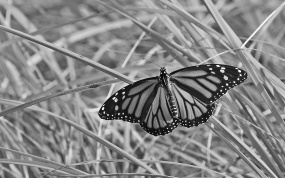
\includegraphics[width=\textwidth]{./figures/box_vs_gaussian_original.jpg}
            \caption{Original}
            \label{sfi:box_vs_gaussian_original}
        \end{subfigure}
        \begin{subfigure}[b]{0.3\textwidth}
            \centering
            
\begin{tikzpicture}[scale=0.2]
            	\coordinate (o) at (0,0);
            	\draw[fill=black!80] (o) ++(-2,-2) rectangle ++(4,4);
            	\draw[fill=black!5] (o) ++(-1,-1) rectangle ++(2,2);
            \end{tikzpicture}
            \caption{Kernel (much zoomed)}
            \label{sfi:box_vs_gaussian_kernel}
        \end{subfigure}
        \begin{subfigure}[b]{0.3\textwidth}
            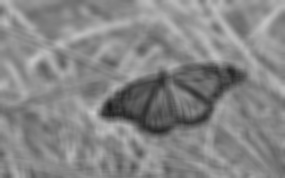
\includegraphics[width=\textwidth]{./figures/box_vs_gaussian_box.jpg}
            \caption{Box Filtered}
            \label{sfi:box_vs_gaussian_box}
        \end{subfigure}
        \caption{Smoothing with Box Filter}\label{fi:smoothing_with_box}
    \end{figure}
    \credit{D. Forsyth}
\end{frame}

\begin{frame}{Box Filter vs. Gaussian Filter}
    \begin{figure}
        \centering
        \begin{subfigure}[b]{0.3\textwidth}
            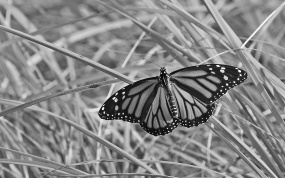
\includegraphics[width=\textwidth]{./figures/box_vs_gaussian_original.jpg}
            \caption{Original}
            \label{sfi:box_vs_gaussian_original}
        \end{subfigure}
        \begin{subfigure}[b]{0.3\textwidth}
            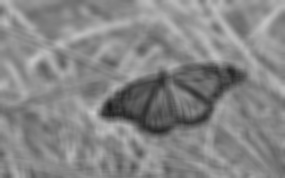
\includegraphics[width=\textwidth]{./figures/box_vs_gaussian_box.jpg}
            \caption{Box Filtered}
            \label{sfi:box_vs_gaussian_box}
        \end{subfigure}
        \begin{subfigure}[b]{0.3\textwidth}
            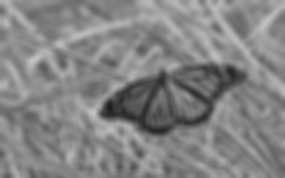
\includegraphics[width=\textwidth]{./figures/box_vs_gaussian_gaussian.jpg}
            \caption{Gaussian Filtered}
            \label{sfi:sharpening_diff}
        \end{subfigure}\\
        \caption{Smoothing with Box and Gaussian Filter}\label{fi:smoothing_with_box_and_gaussian}
    \end{figure}
    \credit{D. Forsyth}
\end{frame}

\begin{frame}{Gaussian Kernel}

    \begin{equation*}
        G_\sigma(x,y) = \frac{1}{2\pi\sigma^2}e^{-\frac{x^2+y^2}{2\sigma^2}}.
    \end{equation*}
    \begin{figure}
        \centering
        \begin{subfigure}[b]{0.3\textwidth}
            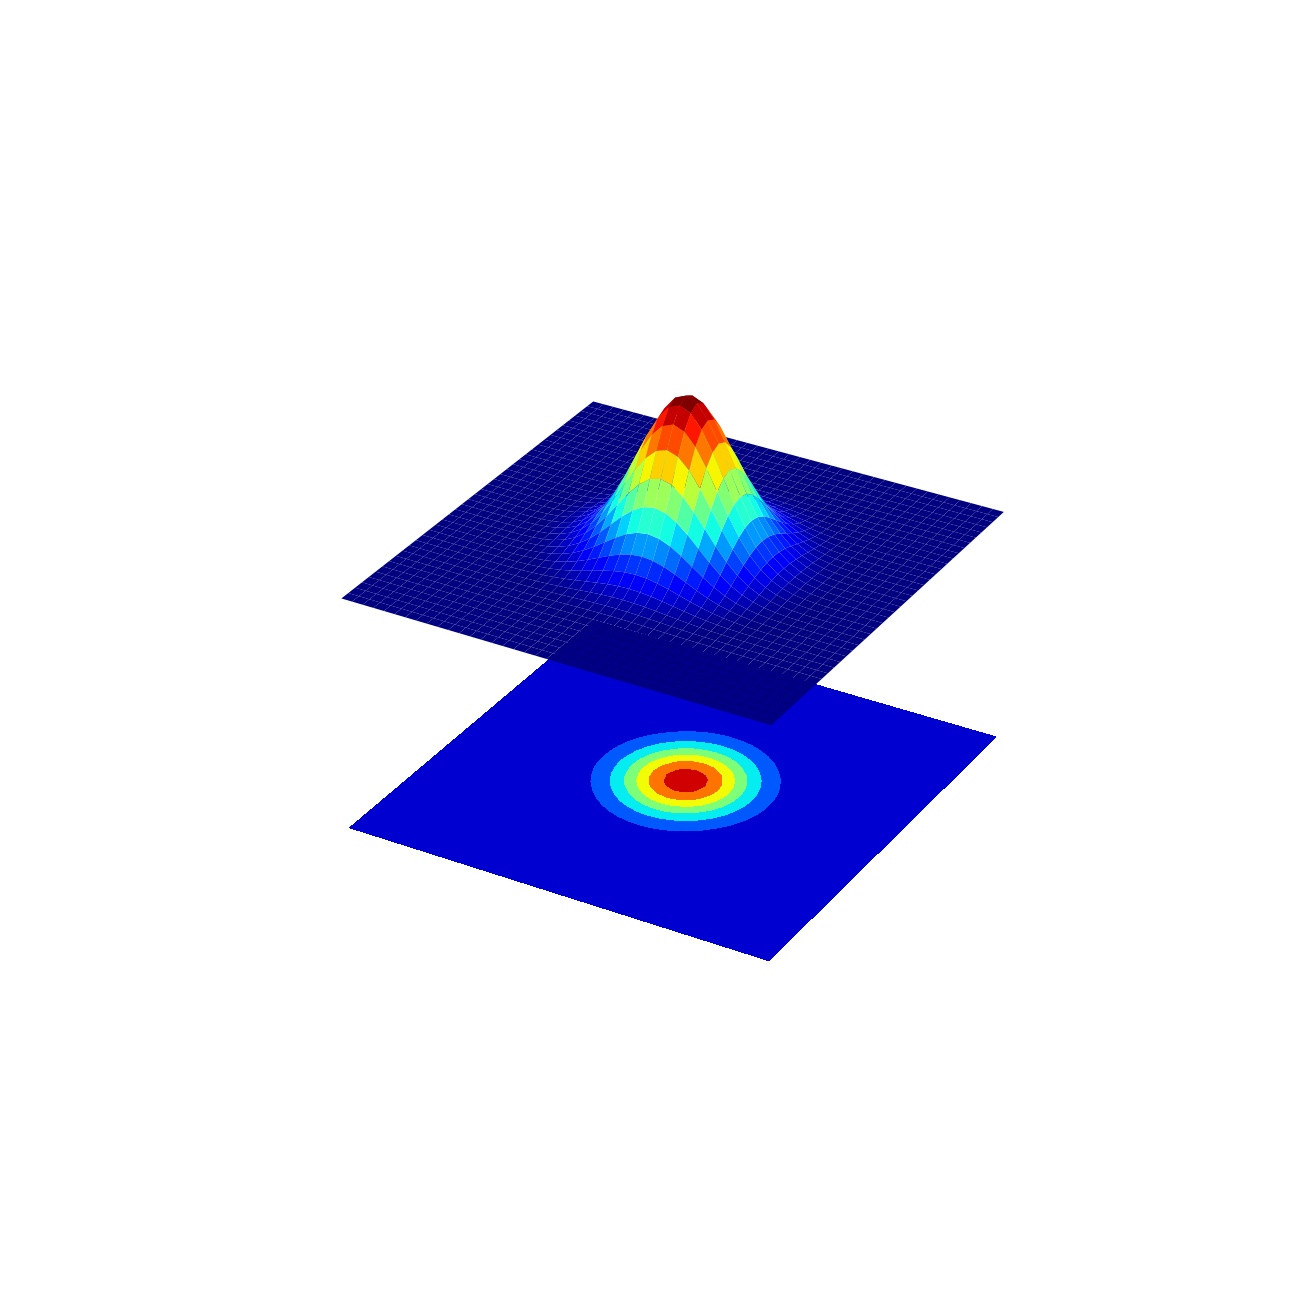
\includegraphics[width=\textwidth, trim={0 300 0 300},clip]{./figures/gaussian_2d_1.jpg}
            %trim={<left> <lower> <right> <upper>}
            \caption{$\sigma = 1$}
            \label{sfi:gaussian_2d_1}
        \end{subfigure}
        \begin{subfigure}[b]{0.3\textwidth}
            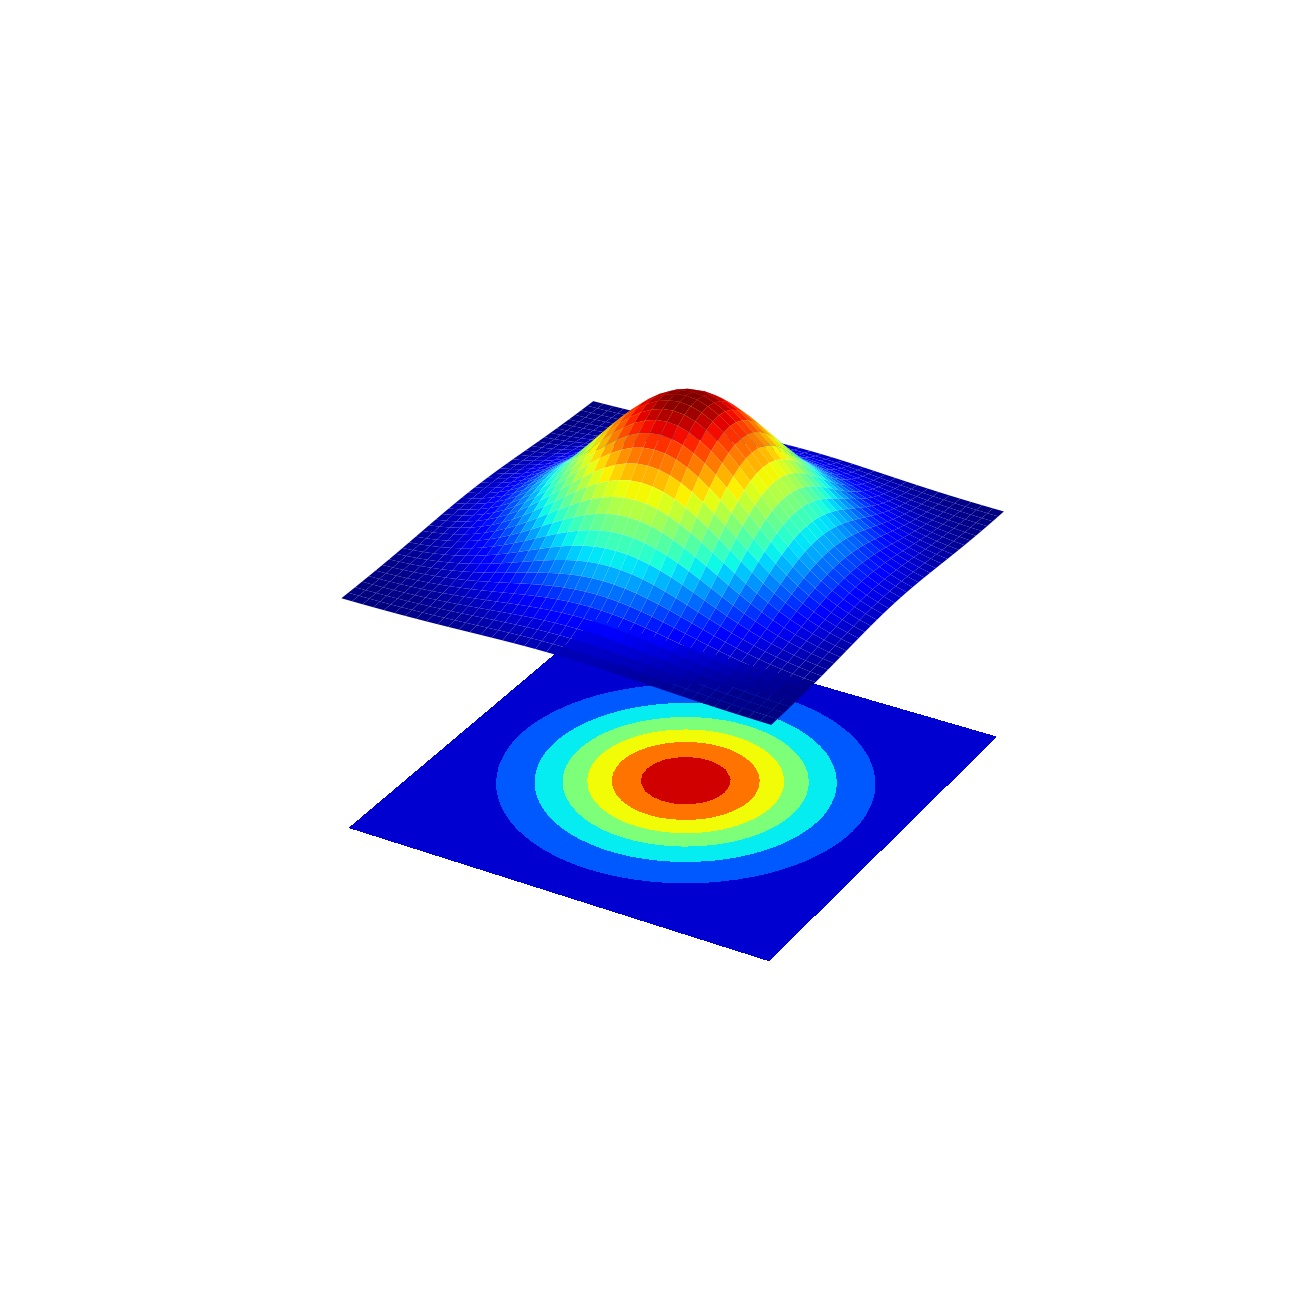
\includegraphics[width=\textwidth, trim={0 300 0 300},clip]{./figures/gaussian_2d_2.jpg}
            \caption{$\sigma = 2$}
            \label{sfi:gaussian_2d_2}
        \end{subfigure}
        \begin{subfigure}[b]{0.3\textwidth}
            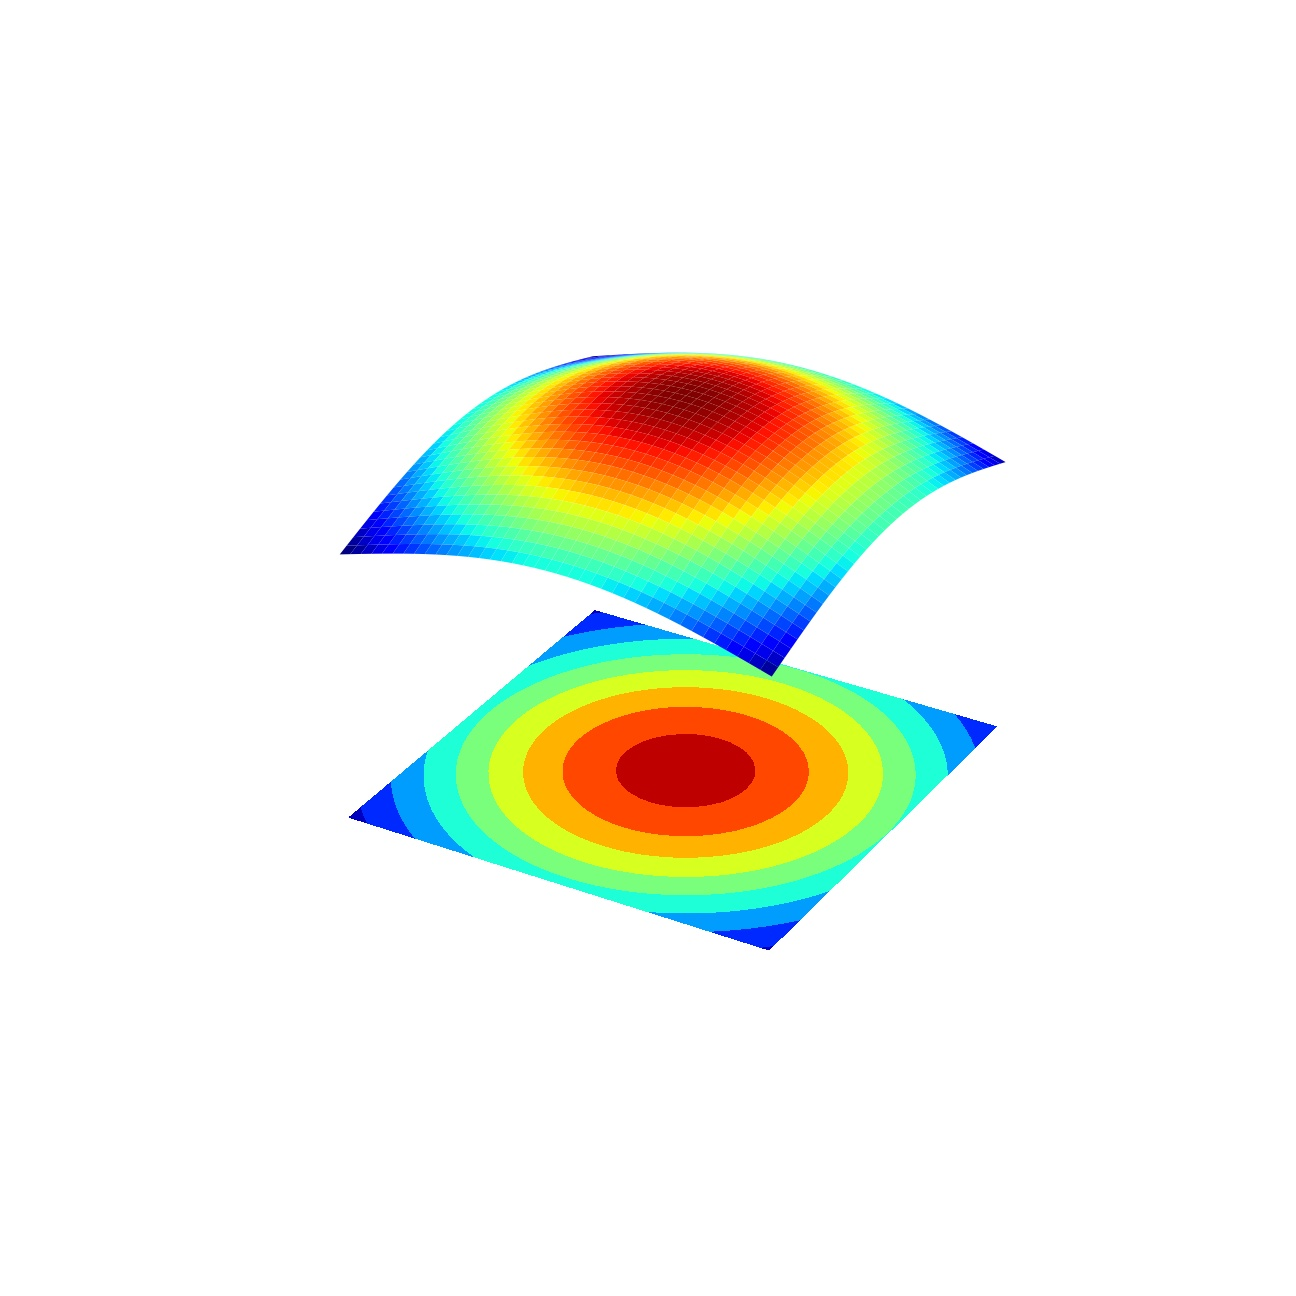
\includegraphics[width=\textwidth, trim={0 300 0 300},clip]{./figures/gaussian_2d_5.jpg}
            \caption{$\sigma = 5$}
            \label{sfi:gaussian_2d_5}
        \end{subfigure}\\
        \caption{2-D Gaussians}\label{fi:gaussians}
    \end{figure}
    \begin{itemize}
      \item Constant factor at front makes volume sum to 1 (can be ignored when computing the filter values, as we should renormalize weights to sum to 1 in any case).
      \item The Gaussian function has infinite support, but discrete filters use finite kernels.
    \end{itemize}



\end{frame}


\begin{frame}[fragile]{Choosing Gaussian Kernel Width}
Rule of thumb: set the filter half-width to about $3\sigma$.
    \pgfmathdeclarefunction{gauss}{2}{%
      \pgfmathparse{1/(#2*sqrt(2*pi))*exp(-((x-#1)^2)/(2*#2^2))}%
    }

    \begin{tikzpicture}
        \begin{axis}[every axis plot post/.append style={
          mark=none,domain=-10:10,samples=50,smooth}, % All plots: from -2:2, 50 samples, smooth, no marks
          axis x line*=bottom, % no box around the plot, only x and y axis
          axis y line*=left, % the * suppresses the arrow tips
          enlargelimits=upper] % extend the axes a bit to the right and top
          \addplot {gauss(0,1)};
          \addlegendentry{$\mu=0, \sigma=1$}
          \addplot {gauss(0,3)};
          \addlegendentry{$\mu=0, \sigma=3$}
          \addplot {gauss(0,5)};
        	\addlegendentry{$\mu=0, \sigma=5$}
        \end{axis}
    \end{tikzpicture}
\end{frame}


%\begin{frame}{Gaussian Filters}
%    \begin{itemize}
%        \item Remove high-frequency components from the image (low-pass filter)
%        \item Convolution with self is another Gaussian
%            \begin{itemize}
%              \item So can smooth with small- kernel, repeat, and get same result as larger-$\sigma$ kernel would have
%              \item Convolving two times with Gaussian kernel with std. dev. $\sigma$ is same as convolving once with kernel with std. dev. $\sigma\sqrt{2}$
%            \end{itemize}
%        \item Separable kernel
%            \begin{itemize}
%              \item Factors into product of two 1D Gaussians
%              \item Discrete example:
%            \end{itemize}
%    \end{itemize}
%
%    \begin{equation*}
%        \begin{bmatrix}
%          1 & 2 & 1 \\
%          2 & 4 & 2 \\
%          1 & 2 & 1
%        \end{bmatrix} =
%        \begin{bmatrix}
%          1 \\
%          2 \\
%          1
%        \end{bmatrix}
%        \begin{bmatrix}
%          1 &
%          2 &
%          1
%        \end{bmatrix}
%    \end{equation*}
%    \credit{K. Grauman}
%\end{frame}

\begin{frame}{Separability of the Gaussian Filter}
    \begin{equation*}
        \begin{split}
        G_\sigma(x,y) &= \frac{1}{2\pi\sigma^2}e^{-\frac{x^2+y^2}{2\sigma^2}},\\
        &= \left[\frac{1}{\sqrt{2\pi}\sigma}e^{-\frac{x^2}{2\sigma^2}}\right]\left[\frac{1}{\sqrt{2\pi}\sigma}e^{-\frac{y^2}{2\sigma^2}}\right].\\
        \end{split}
    \end{equation*}
    \begin{itemize}
        \item The 2-D Gaussian can be expressed as the product of two functions, one a function of $x$ and the other a function of $y$.
        \item In this case, the two Gaussians are the (identical) 1-D Gaussians.
        \pause
        \item Separability means that a 2-D convolution can be reduced to two 1-D convolutions (one among rows and one among columns).
        \item What is the complexity of filtering an $n\times n$ image with an $m\times m$ kernel?\pause \fillblank{$O(n^2m^2)$}.
        \item What is the complexity if the kernel is separable?\pause \fillblank{$O(n^2m)$}.
    \end{itemize}
    \credit{D. Forsyth}
\end{frame}
